% this file is called up by thesis.tex
% content in this file will be fed into the main document

%: ----------------------- name of chapter  -------------------------
\chapter{Title} % top level followed by section, subsection
%Towards simplyfing user's authentication in mobile apps.

In Chapter 2 multiple alternatives to automating authentication were discussed. This section will focus on the solution developed as part of this theses. 


%: ----------------------- paths to graphics ------------------------

% change according to folder and file names
\ifpdf
    \graphicspath{{X/figures/PNG/}{X/figures/PDF/}{X/figures/}}
\else
    \graphicspath{{X/figures/EPS/}{X/figures/}}
\fi

%: ----------------------- Mobile Cloud Middleware ------------------------

\section{Short description of the solution}
This solution provides a library that developers can apply in their applications with very little coding. All needed to do is import the library into a project and refer to it.

The library provides easy registration for new credentials, storing them and retrieving for authentication. The user only inserts the credentials once and protects them with a pattern which is used for retrieving them. The pattern and the credentials are stored locally in a database, which is application specific and can only be accessed by it. 

An example project is used in this paper for demonstration purposes.

\newpage

\section{Android lockpattern}
\begin{wrapfigure}{r}{0.4\textwidth} 
\begin{center} 
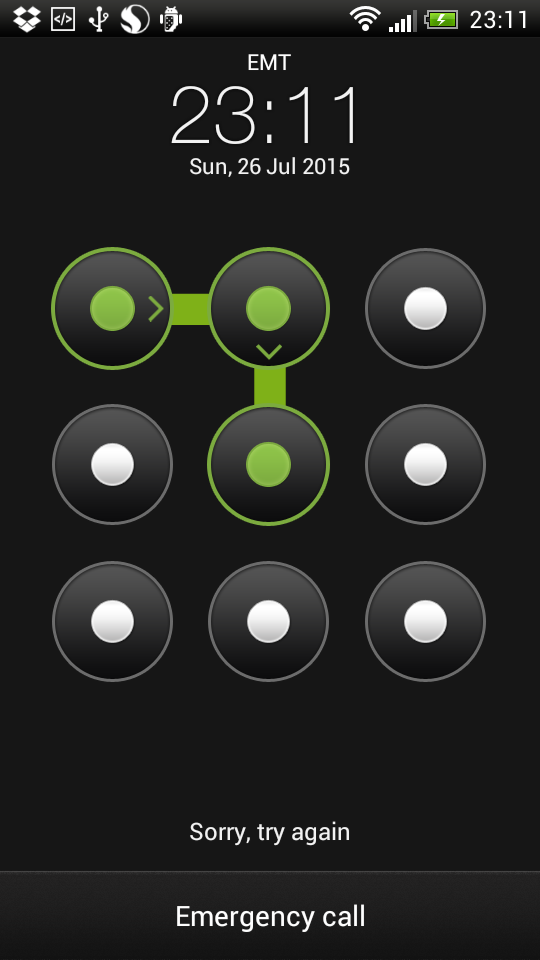
\includegraphics[width=0.35\textwidth]{images/lockpattern.png} \caption{Android lockpattern} \label{fig:android lockpattern} 
\end{center}
\end{wrapfigure}
As mentioned in the previous section a pattern is used to protect the credentials. Android users might already be familiar with the lockpattern even when they have not heard the term itself. It is used for locking the device from unwanted access to it, shown in the Figure 4.1. It is a 3x3 matrix consisting of circles/dots. To draw a pattern a user must press on a circle and drag through others to make a pattern and release to verify it. Even though the user only sees a picture of the pattern it is actually a string of numbers representing the dots where the user changed direction. For example a string "1-7-8" would be a pattern "L". 
Android lockpattern is known to users and is very easy to understand. Typing is taken out of the authentication process, which reduces the amount of errors made, and therefore used in this solution.

\section{Supporting Multiple Users}
The key factor what makes it different from previous solutions is the support for multiple users and multiple accounts per user. Mobile devices are commonly personal, but tablets in the other hand could be used in a household by the whole family. Needless to say that having to authenticate numerous times during a day might be a pain. 

\section{Data storage}
Every android comes with built in database system - SQLite \footnote[8]{https://www.sqlite.org/}. It is easy to use, yet powerful to handle large amounts of data. Though no device will ever have the amount of users to even slightly test the database system, the benefit of using it is the simplicity and scalability allowing future changes in the database without losing any data already stored.

Since the library itself does not directly save data or query for it from the database, an Android component Content Provider \footnote[9]{http://developer.android.com/intl/zh-CN/reference/android/content/ContentProvider.html} is used. It manages access to the data, encapsulates it and provides mechanisms for defining data security. Content Providers can be used in two ways: provide access to it for all applications or just the one with permissions. In this case only the application intended to use it is given permissions declining any intruders from sniffing around.

\section{Structure of the library}
This section will go more specific into the structure, classes and flow of the library to give insight of how it works.

As mentioned numerous times previously, this solution is a library for Android applications. To be effective in the world of coding, reusing code made by self or others is essential. The same rule is implied here by using a library that withdraws the lockpattern function from Android source code. That is to say amongst other libraries used to create the final product of an application, these two libraries would be used in an application component tree as shown in the Figure 4.2.

\begin{figure}[h]
\begin{center}
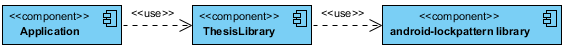
\includegraphics[scale=0.9]{images/componentdiagram.png}
\caption{Example of application component diagram} \label{fig:component diagram} 
\end{center}
\end{figure}

The code within the library is somewhat sectioned: interface to the library, activities/visual presentation, content provider and database management. The most substantiate part of the code is database management with the highest complexity giving  the library flexibility. The database currently is located internally in the device, but the code is designed to allow moving it to another path on the device or entirely off to a cloud. All the data columns are defined in a "database contract" for easy access and modification, the database will automatically update itself if the underlying data model is changed and using singleton pattern only one instance of the database can run at any given time to prevent data corruption. The database management classe including the other classe can be seen in the class diagram in the Figure 4.3.

The code within the library can also be divided into sections: interface to the library, activities/visual presentation, content provider and database management. It may seem much for so trivial task, every little component serves its purpose to 

Though applications and libraries are developed for present requirements, the future can not be foreseen and should always be somewhat considered. To make this library flexible to unseen changes design patterns are used. 

\begin{landscape}

\begin{figure}[h]
\begin{center}
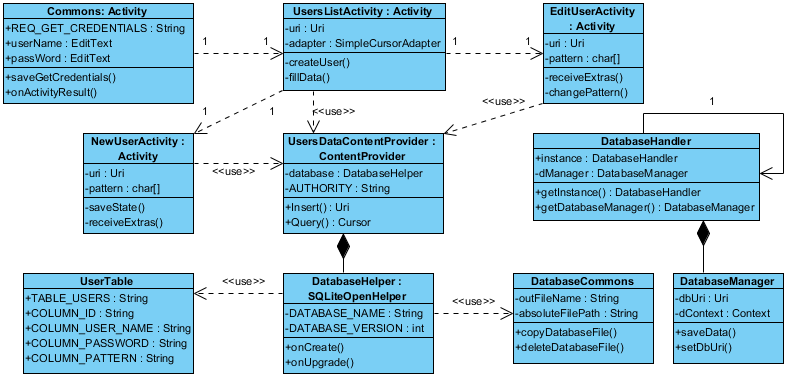
\includegraphics[scale=1.1]{images/classdiagram.png}
\caption{Class diagram of the library} \label{fig:class diagram} 
\end{center}
\end{figure}

\end{landscape}

\newpage

\section{Flow of the library}
To better understand what the library does, it is good to know the flow of it. For better visualisation a few diagrams are used.

Often less is more, this is the design ideal behind the library. A user has two main actions that he will take to authenticate: register an a account and start authenticating with it. In other words, one action is to get the credentials of the account into the phones memory and the other to access them.
 
When a user is logging into an application, using this library, he is asked whether he would like to save the credentials. If so he is taken to an activity to verify the password once more. When the password is verified, a new activity is presented to create a pattern for future authentication, and finally the credentials with the newly created pattern are stored to the database. This procedure is also illustrated on Figure 4.4 as a sequence diagram.

\begin{figure}[h]
\begin{center}
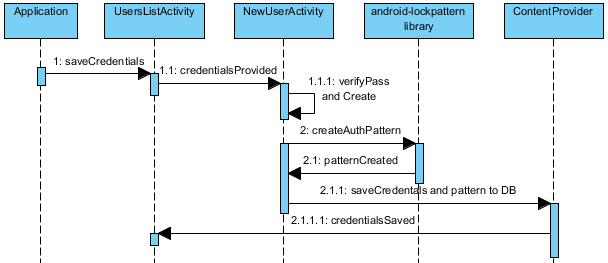
\includegraphics[scale=0.9]{images/sequencediagramnew.png}
\caption{Sequence diagram of registrating new account} \label{fig:sequence diagram} 
\end{center}
\end{figure}

With one or more credentials stored in the database the user can authenticate using them. Either finishing the registration sequence or accessing the UsersListAcivity from the the application, the user has a list of stored credentials presented to him. Clicking on a chosen account the library will get the information from the database and ask the user to verify the account by inputting the pattern. On a successful verification the credentials are passed to the application. Illustrative sequence diagram is shown on the Figure 4.5.

\begin{figure}[h!]
\begin{center}
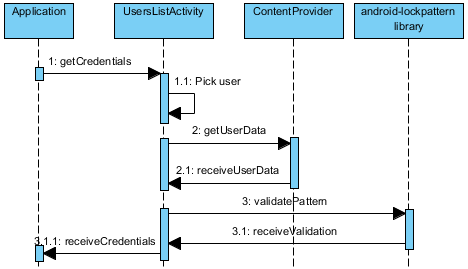
\includegraphics[scale=0.9]{images/sequencediagramauth.png}
\caption{Sequence diagram of authentication} \label{fig:sequence diagram} 
\end{center}
\end{figure}

\newpage
The previous descriptions and sequence diagrams of the registration and authentication process give the idea of a successful interpretation of the library. Though the user is given choices to back out of the process or the process could be failed. A flow chart covering these possibilities is seen in the Figure 4.6.

\begin{figure}[h!]
\begin{center}
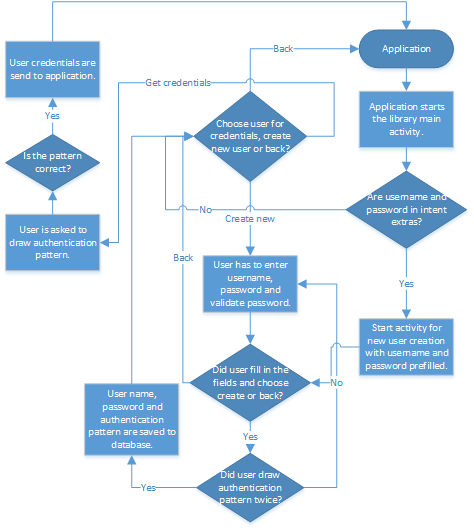
\includegraphics[scale=1.2]{images/flowchart.png}
\caption{Flow chart of registration and authentication process} 
\label{fig:flow chart} 
\end{center}
\end{figure}

\newpage

\section{Importing the library into a project}
This section is describing how to include this library in a project in terms of getting the library in a workspace and the code necessary to run it. 

In order to use this library, both this and the Android-Lockpattern library are needed. This library is accessible in the projects repository \footnote[10]{https://github.com/ennoeller/ThesisApi}, and also Android-Lockpatter library is accessible on github \footnote[11]{https://github.com/haibison/android-lockpattern}. For development, eclipse is needed, as these libraries only work there. Within eclipse, both libraries have to be imported as projects, alongside with application project, which will include them. 

In order for the library to work, a few lines of code have to be added to the application project. One row needs to be added to the project properties file, also make sure that a reference to the library is there:

\begin{lstlisting}
manifestmerger.enabled=true
android.library.reference.1=../ThesisApi
\end{lstlisting} 
	
Example usage of the library in an activity would look something like this:

\lstset{language=Java}

\begin{lstlisting}
import thesis.thesis.Commons;

public class Main extends Commons {

    @Override
	protected void onCreate(Bundle savedInstanceState) {
		super.onCreate(savedInstanceState);
		setContentView(R.layout.activity_main);

		userName = (EditText) findViewById(R.id.username);
		passWord = (EditText) findViewById(R.id.password);
		
		Button bCallLibrary = (Button) findViewById(R.id.bCallLibrary);
		bCallLibrary.setOnClickListener(new View.OnClickListener() {
			public void onClick(View v) {

				saveGetCredentials(userName.getText().toString(), passWord.getText().toString());
			}
		});	
	}
}
\end{lstlisting}




\section{Summary}
A new mechanism for authentication was developed as a library for Android. It uses patterns and therefore is very easy to use and also supports multiple users. For the end users the flow is kept minimalistic to increase simplicity and transparency. Use in a project is made very simple with an interface, as can be seen from the sample code. 

The next chapter discusses the method used for gathering feedback and analyses the results. 



% ---------------------------------------------------------------------------
%: ----------------------- end of thesis sub-document ------------------------
% ---------------------------------------------------------------------------

